\documentclass[12pt]{article}
\usepackage[T1]{fontenc}
\usepackage{lmodern}
\usepackage{amssymb,amsmath}
\usepackage{ifxetex,ifluatex}
\usepackage{fixltx2e} % provides \textsubscript
% use upquote if available, for straight quotes in verbatim environments
\IfFileExists{upquote.sty}{\usepackage{upquote}}{}
\ifnum 0\ifxetex 1\fi\ifluatex 1\fi=0 % if pdftex
  \usepackage[utf8]{inputenc}
\else % if luatex or xelatex
  \ifxetex
    \usepackage{mathspec}
    \usepackage{xltxtra,xunicode}
  \else
    \usepackage{fontspec}
  \fi
  \defaultfontfeatures{Mapping=tex-text,Scale=MatchLowercase}
  \newcommand{\euro}{€}
\fi
% use microtype if available
\IfFileExists{microtype.sty}{\usepackage{microtype}}{}
\usepackage{color}
\usepackage{fancyvrb}
\newcommand{\VerbBar}{|}
\newcommand{\VERB}{\Verb[commandchars=\\\{\}]}
\DefineVerbatimEnvironment{Highlighting}{Verbatim}{commandchars=\\\{\}}
% Add ',fontsize=\small' for more characters per line
\usepackage{framed}
\definecolor{shadecolor}{RGB}{248,248,248}
\newcommand{\KeywordTok}[1]{\textcolor[rgb]{0.13,0.29,0.53}{\textbf{{#1}}}}
\newcommand{\DataTypeTok}[1]{\textcolor[rgb]{0.13,0.29,0.53}{{#1}}}
\newcommand{\DecValTok}[1]{\textcolor[rgb]{0.00,0.00,0.81}{{#1}}}
\newcommand{\BaseNTok}[1]{\textcolor[rgb]{0.00,0.00,0.81}{{#1}}}
\newcommand{\FloatTok}[1]{\textcolor[rgb]{0.00,0.00,0.81}{{#1}}}
\newcommand{\CharTok}[1]{\textcolor[rgb]{0.31,0.60,0.02}{{#1}}}
\newcommand{\StringTok}[1]{\textcolor[rgb]{0.31,0.60,0.02}{{#1}}}
\newcommand{\CommentTok}[1]{\textcolor[rgb]{0.56,0.35,0.01}{\textit{{#1}}}}
\newcommand{\OtherTok}[1]{\textcolor[rgb]{0.56,0.35,0.01}{{#1}}}
\newcommand{\AlertTok}[1]{\textcolor[rgb]{0.94,0.16,0.16}{{#1}}}
\newcommand{\FunctionTok}[1]{\textcolor[rgb]{0.00,0.00,0.00}{{#1}}}
\newcommand{\RegionMarkerTok}[1]{{#1}}
\newcommand{\ErrorTok}[1]{\textbf{{#1}}}
\newcommand{\NormalTok}[1]{{#1}}
\usepackage{graphicx}
% Redefine \includegraphics so that, unless explicit options are
% given, the image width will not exceed the width of the page.
% Images get their normal width if they fit onto the page, but
% are scaled down if they would overflow the margins.
\makeatletter
\def\ScaleIfNeeded{%
  \ifdim\Gin@nat@width>\linewidth
    \linewidth
  \else
    \Gin@nat@width
  \fi
}
\makeatother
\let\Oldincludegraphics\includegraphics
{%
 \catcode`\@=11\relax%
 \gdef\includegraphics{\@ifnextchar[{\Oldincludegraphics}{\Oldincludegraphics[width=\ScaleIfNeeded]}}%
}%
\ifxetex
  \usepackage[setpagesize=false, % page size defined by xetex
              unicode=false, % unicode breaks when used with xetex
              xetex]{hyperref}
\else
  \usepackage[unicode=true]{hyperref}
\fi
\hypersetup{breaklinks=true,
            bookmarks=true,
            pdfauthor={},
            pdftitle={},
            colorlinks=true,
            citecolor=blue,
            urlcolor=blue,
            linkcolor=magenta,
            pdfborder={0 0 0}}
\urlstyle{same}  % don't use monospace font for urls
\setlength{\parindent}{0pt}
\setlength{\parskip}{6pt plus 2pt minus 1pt}
\setlength{\emergencystretch}{3em}  % prevent overfull lines
\setcounter{secnumdepth}{0}
\usepackage{fullpage}
\usepackage{framed}
\usepackage{mathtools}
\usepackage[osf]{mathpazo} % palatino
\usepackage{float}

\begin{document}

\title{Phylogenetic Comparative Methods in R\\
Using phylogeny as a statistical fix}
\author{Natalie Cooper (ncooper@tcd.ie)}
\date{}
\maketitle

The aims of this problem set are to learn how to use R to answer phylogenetic 
comparative questions without panicking! I am assuming that people have little or no
experience with R so more experienced users may want to skip quickly through the first 
few sections. By the end of this problem set you should be able to:

\begin{enumerate}
\item Read your data and phylogeny into R
\item View and manipulate your data and phylogeny
\item Match taxa in your data with those in your phylogeny
\item Perform PGLS analyses using \texttt{caper}
\item Perform model diagnostics for PGLS
\item Estimate phylogenetic signal using $\lambda$ and K
\end{enumerate}

We will be using the evolution of primate life-history variables as an
example. These data come from the PanTHERIA database (Jones \textit{et
al}. 2009) and 10kTrees (Arnold \textit{et al}. 2010). Note that this is
an old version of 10kTrees, so if you want to use it in your research
please download the newest version.

Throughout, R code will be in shaded boxes:

\begin{snugshade}
\begin{Highlighting}[]
\KeywordTok{install.packages}\NormalTok{(}\StringTok{"ape"}\NormalTok{)}
\end{Highlighting}
\end{snugshade}

R output will be preceded by \texttt{\#\#} and important comments will be in boxes:

\begin{framed}
Note that many things in R can be done in multiple ways. You should
choose the methods you feel most comfortable with, and do not panic if
someone is doing the same analyses as you in a different way! This
workshop will be full of different ways to do things.
\end{framed}

\newpage{}
\section{Preparations}

\subsection{Downloading the data and finding the path of your folder}

First you need to download all the files for this problem set into a
folder somewhere on your computer, let's call it ``RAnalyses2014'' and
pop it on the Desktop. We will use this folder throughout the problem
set. You'll need to know what the \textbf{path} of the folder is. For
example on my Windows machine, the path is:

\begin{snugshade}
\texttt{C:/Users/Natalie/Desktop/RAnalyses2014}
\end{snugshade}

The path is really easy to find in a Windows machine, just click on the
address bar of the folder and the whole path will appear.

\begin{framed}
In Windows, paths usually include \textbackslash{} but R
can't read these. It's easy to fix in your R code, just change any \textbackslash{} in
the path to / or \textbackslash{}\textbackslash{}.
\end{framed}

On my Mac the path is:

\begin{snugshade}
\texttt{\textasciitilde{}/Desktop/RAnalyses2014}
\end{snugshade}

It's a bit trickier to find the path on a Mac, and note that the tilde
\textasciitilde{} is a shorthand for /Users/Natalie. Ask if you need help.

\subsection{Using a text editor}

Next, open a text editor. R has an inbuilt editor that works pretty
well, but NotePad and TextEdit are fine too. However, in the future I
\textbf{highly} recommend using something that will highlight code for
you. My personal favorite is Sublime Text 2, because you can also use
it for any other kind of text editing like LaTeX, html etc.

You should type (or copy and paste) your code into the text editor, edit
it until you think it'll work, and then paste it into R's console
window. Saving the text file lets you keep a record of the code you
used, which can be a great timesaver if you want to use it again,
especially as you know this code will work!

\begin{framed}
You can cut and paste code from this handout into your text editor, or straight into R. You don't need to retype everything!
\end{framed}

If you want to add comments to the file (i.e., notes to remind yourself
what the code is doing), put a hash/pound sign (\#) in front of the
comment.

\begin{snugshade}
\texttt{\# Comments are ignored by R but can remind you what the code is doing.\\}
\texttt{\# You need a hash sign at the start of each line of a comment.}
\end{snugshade}

\subsection{Installing extra packages in R}\label{installing-packages}

To run comparative analyses (or any specialised analysis) in R, you need to 
download one or more additional packages from the basic R installation. 
For this problems set you will need to install the following packages: 
\texttt{ape}, \texttt{picante} and \texttt{caper}. 
To install the package \texttt{ape}:

\begin{snugshade}
\begin{Highlighting}[]
\KeywordTok{install.packages}\NormalTok{(}\StringTok{"ape"}\NormalTok{)}
\end{Highlighting}
\end{snugshade}

Now install \texttt{picante} and \texttt{caper}.

\subsection{Loading packages in R}

You've installed the packages but they don't automatically get loaded
into your R session. Instead you need to tell R to load them \textbf{every
time} you start a new R session and want to use functions from these
packages. To load the package \texttt{ape} into your current R session:

\begin{snugshade}
\begin{Highlighting}[]
\KeywordTok{library}\NormalTok{(ape)}
\end{Highlighting}
\end{snugshade}

Don't forget to load \texttt{picante} and \texttt{caper} too!

\newpage
\section{Reading your data and phylogeny into R}
\subsection{Reading data into R}

Next we need to load the data we are going to use for the analysis. R
can read files in lots of formats, including comma-delimited and
tab-delimited files. Excel (and many other applications) can output
files in this format (it's an option in the ``Save As'' dialog box
under the ``File'' menu). To save time I have given you a tab-delimited
text file called ``Primatedata.txt'' which we are going to use. Load
these data as follows. 

\begin{framed}
You will need to replace MYPATH with the name of the path to the folder containing the data and tree on your computer.
\end{framed}

\begin{snugshade}
\begin{Highlighting}[]
\NormalTok{primatedata <-}\StringTok{ }\KeywordTok{read.table}\NormalTok{(}\StringTok{"MYPATH/Primatedata.txt"}\NormalTok{, }\DataTypeTok{sep =} \StringTok{"}\CharTok{\textbackslash{}t}\StringTok{"}\NormalTok{, }\DataTypeTok{header =} \OtherTok{TRUE}\NormalTok{)}
\end{Highlighting}
\end{snugshade}

Note that \texttt{sep = "\textbackslash{}t"} indicates that you have a tab-delimited file, 
\texttt{sep = ","}  would indicate a comma-delimited csv file. You can also use
\texttt{read.delim} for tab delimited files or \texttt{read.csv} for comma delimited
files. \texttt{header = TRUE}, indicates that the first line of the data contains
column headings.

This is a good point to note that unless you \textbf{tell} R you want to
do something, it won't do it automatically. So here if you successfully
entered the data, R won't give you any indication that it worked.
Instead you need to specifically ask R to look at the data.

We can look at the data by typing:

\begin{snugshade}
\begin{Highlighting}[]
\KeywordTok{str}\NormalTok{(primatedata)}
\end{Highlighting}
\end{snugshade}

\begin{verbatim}
## 'data.frame':    77 obs. of  8 variables:
##  $ Order          : Factor w/ 1 level "Primates": 1 1 1 ...
##  $ Family         : Factor w/ 15 levels "Aotidae","Atelidae",...
##  $ Binomial       : Factor w/ 77 levels "Alouatta palliata",...
##  $ AdultBodyMass_g: num  6692 7582 8697 958 558 ...
##  $ GestationLen_d : num  138 226 228 164 154 ...
##  $ HomeRange_km2  : num  2.28 0.73 1.36 0.02 0.32 0.02 ...
##  $ MaxLongevity_m : num  336 328 454 304 215 ...
##  $ SocialGroupSize: num  14.5 42 20 2.95 6.85 ...
\end{verbatim}

This shows the structure of the data frame (this can be a really useful
command when you have a big data file). It also tells you what kind of
variables R thinks you have (characters, integers, numeric, factors
etc.). Some R functions need the data to be certain kinds of variables
so it's useful to check this.

As you can see, the data contains the following variables: Order,
Family, Binomial, AdultBodyMass\_g, GestationLen\_d, HomeRange\_km2,
MaxLongevity\_m, and SocialGroupSize.

\begin{snugshade}
\begin{Highlighting}[]
\KeywordTok{head}\NormalTok{(primatedata)}
\end{Highlighting}
\end{snugshade}

\begin{verbatim}
##      Order      Family           Binomial AdultBodyMass_g GestationLen_d
## 1 Primates    Atelidae   Ateles belzebuth          6692.4          138.2
## 2 Primates    Atelidae   Ateles geoffroyi          7582.4          226.4
## 3 Primates    Atelidae    Ateles paniscus          8697.2          228.2
## 4 Primates Pitheciidae  Callicebus moloch           958.1          164.0
## 5 Primates     Cebidae  Callimico goeldii           558.0          154.0
## 6 Primates     Cebidae Callithrix jacchus           290.2          144.0
##   HomeRange_km2 MaxLongevity_m SocialGroupSize
## 1          2.28          336.0           14.50
## 2          0.73          327.6           42.00
## 3          1.36          453.6           20.00
## 4          0.02          303.6            2.95
## 5          0.32          214.8            6.85
## 6          0.02          201.6            8.55
\end{verbatim}

This gives you the first few rows of data along with the column
headings.

\begin{snugshade}
\begin{Highlighting}[]
\KeywordTok{names}\NormalTok{(primatedata)}
\end{Highlighting}
\end{snugshade}

\begin{verbatim}
## [1] "Order"           "Family"          "Binomial"        "AdultBodyMass_g"
## [5] "GestationLen_d"  "HomeRange_km2"   "MaxLongevity_m"  "SocialGroupSize"
\end{verbatim}

This gives you the names of the columns.

\begin{snugshade}
\begin{Highlighting}[]
\NormalTok{primatedata}
\end{Highlighting}
\end{snugshade}

This will print out the whole of the data!

\subsection{Reading and displaying your phylogeny in R}

To load a tree you need either the function \texttt{read.tree} or \texttt{read.nexus}.
\texttt{read.tree} can deal with a number of different types of data (including
DNA) whereas \texttt{read.nexus} reads NEXUS files. We will use a NEXUS file of
the consensus tree from 10kTrees.

\begin{framed}
You will need to replace MYPATH with the name of the path to the folder containing the data and tree on your computer.
\end{framed}

\begin{snugshade}
\begin{Highlighting}[]
\NormalTok{primatetree <-}\StringTok{ }\KeywordTok{read.nexus}\NormalTok{(}\StringTok{"MYPATH/consensusTree_10kTrees_Version2.nex"}\NormalTok{)}
\end{Highlighting}
\end{snugshade}

Let's examine the tree by typing:

\begin{snugshade}
\begin{Highlighting}[]
\NormalTok{primatetree}
\end{Highlighting}
\end{snugshade}

\begin{verbatim}
## Phylogenetic tree with 226 tips and 221 internal nodes.
## 
## Tip labels:
##  Allenopithecus_nigroviridis, Cercopithecus_ascanius, 
Cercopithecus_cephus, Cercopithecus_cephus_cephus, ...
## 
## Rooted; includes branch lengths.
\end{verbatim}

\begin{snugshade}
\begin{Highlighting}[]
\KeywordTok{str}\NormalTok{(primatetree)}
\end{Highlighting}
\end{snugshade}

\begin{verbatim}
## List of 4
##  $ edge       : int [1:446, 1:2] 227 228 229 230 231 232 ...
##  $ edge.length: num [1:446] 4.95 17.69 19.65 8.12 4.82 ...
##  $ Nnode      : int 221
##  $ tip.label  : chr [1:226] "Allenopithecus_nigroviridis" ...
##  - attr(*, "class")= chr "phylo"
##  - attr(*, "order")= chr "cladewise"
\end{verbatim}

\texttt{primatetree} is a fully resolved tree with branch lengths. There are 226
species and 221 internal nodes. We can plot the tree by using the \texttt{plot}
function of \texttt{ape}:

\begin{snugshade}
\begin{Highlighting}[]
\KeywordTok{plot}\NormalTok{(primatetree}\NormalTok{)}
\end{Highlighting}
\end{snugshade}

Note that the tree is too large to read. You can make the node labels smaller, but that doesn’t help much here:

\begin{snugshade}
\begin{Highlighting}[]
\KeywordTok{plot}\NormalTok{(primatetree, }\DataTypeTok{cex =} \FloatTok{0.5}\NormalTok{)}
\end{Highlighting}
\end{snugshade}

Alternatively you can zoom into different sections of the tree which you’re interested in:

\begin{snugshade}
\begin{Highlighting}[]
\KeywordTok{zoom}\NormalTok{(primatetree, }\KeywordTok{list}\NormalTok{(}\KeywordTok{grep}\NormalTok{(}\StringTok{"Cercopithecus"}\NormalTok{, primatetree\$tip.label)), }
      \DataTypeTok{subtree =} \OtherTok{FALSE}\NormalTok{)}
\end{Highlighting}
\end{snugshade}

This just gives you the tree for \textit{Cercopithecus} species but you can also see how the species fit into the rest of the tree using:

\begin{snugshade}
\begin{Highlighting}[]
\KeywordTok{zoom}\NormalTok{(primatetree, }\KeywordTok{list}\NormalTok{(}\KeywordTok{grep}\NormalTok{(}\StringTok{"Cercopithecus"}\NormalTok{, primatetree\$tip.label)), }
      \DataTypeTok{subtree =} \OtherTok{TRUE}\NormalTok{)}
\end{Highlighting}
\end{snugshade}

Note that \texttt{zoom} automatically sets the plotting window to display two plots at once. To reset this to one plot only use:

\begin{snugshade}
\begin{Highlighting}[]
\KeywordTok{par}\NormalTok{(}\DataTypeTok{mfrow =} \KeywordTok{c}\NormalTok{(}\DecValTok{1}\NormalTok{, }\DecValTok{1}\NormalTok{))}
\end{Highlighting}
\end{snugshade}

You can also remove species from the tree very easily using the \texttt{ape} function \texttt{drop.tip}:

\begin{snugshade}
\begin{Highlighting}[]
\NormalTok{primatetree2 <-}\StringTok{ }\KeywordTok{drop.tip}\NormalTok{(primatetree, }\StringTok{"Aotus_azarae_infulatus"}\NormalTok{)}
\KeywordTok{str}\NormalTok{(primatetree2)}
\end{Highlighting}
\end{snugshade}

\begin{verbatim}
## List of 4
##  $ edge       : int [1:444, 1:2] 226 227 228 229 ...
##  $ edge.length: num [1:444] 4.95 17.69 19.65 8.12 ...
##  $ Nnode      : int 220
##  $ tip.label  : chr [1:225] "Allenopithecus_nigroviridis" ...
##  - attr(*, "class")= chr "phylo"
##  - attr(*, "order")= chr "cladewise"
\end{verbatim}

To remove more than one species see below. To get further options for the plotting of phylogenies:

\begin{snugshade}
\begin{Highlighting}[]
\DataTypeTok{?}\NormalTok{(plot.phylo)}
\end{Highlighting}
\end{snugshade}

Note that although you can use \texttt{plot} to plot the phylogeny, you need to specify \texttt{plot.phylo} to find out the options for plotting trees. You can change the style of the tree (type), the color of the branches and tips (edge.color, tip.color). Here’s an fun example! 

\begin{snugshade}
\begin{Highlighting}[]
\KeywordTok{par}\NormalTok{(}\DataTypeTok{mfrow =} \KeywordTok{c}\NormalTok{(}\DecValTok{1}\NormalTok{, }\DecValTok{1}\NormalTok{))}
\KeywordTok{plot}\NormalTok{(primatetree, }\DataTypeTok{type =} \StringTok{"fan"}\NormalTok{, }\DataTypeTok{edge.color =} \StringTok{"deeppink"}\NormalTok{, }\DataTypeTok{tip.color =} 
      \StringTok{"green"}\NormalTok{, }\DataTypeTok{cex =} \FloatTok{0.5}\NormalTok{)}
\end{Highlighting}
\end{snugshade}

You can also add a timescale to your tree:

\begin{snugshade}
\begin{Highlighting}[]
\KeywordTok{plot}\NormalTok{(primatetree)}
\KeywordTok{axisPhylo}\NormalTok{()}
\end{Highlighting}
\end{snugshade}

Most R functions require your tree to be dichotomous, i.e. to have no polytomies. To check whether your tree is dichotomous use \texttt{is.binary.tree}. If this is FALSE, use \texttt{multi2di} to make the tree dichotomous. This function works by randomly resolving polytomies with zero-length branches.

\begin{snugshade}
\begin{Highlighting}[]
\KeywordTok{is.binary.tree}\NormalTok{(primatetree)}\CommentTok{# we want this to be TRUE}
\end{Highlighting}
\end{snugshade}

\begin{verbatim}
## [1] FALSE
\end{verbatim}

\begin{snugshade}
\begin{Highlighting}[]
\NormalTok{primatetree <-}\StringTok{ }\KeywordTok{multi2di}\NormalTok{(primatetree)}
\end{Highlighting}
\end{snugshade}

Most functions also require the tree to be rooted, i.e., to have one taxon designated as the outgroup. Our tree is rooted but if you wanted to change the root, or root an unrooted tree use \texttt{root}. Note that here I've just chosen a random species (\textit{Saimiri sciureus}) to be the root.

\begin{snugshade}
\begin{Highlighting}[]
\NormalTok{primatetree.reroot <-}\StringTok{ }\KeywordTok{root}\NormalTok{(primatetree, }\StringTok{"Saimiri_sciureus"}\NormalTok{)  }
\KeywordTok{plot}\NormalTok{(primatetree.reroot)}
\end{Highlighting}
\end{snugshade}

\subsection{Manipulating your data and phylogeny in R}

\subsubsection{Species names with spaces} 
Species names in the tree cannot contain spaces so they are generally written as Genus\_species (the gap between the genus name and species name replaced by \_). If the species names in the data are written as Genus species with a space, then you will have to replace the spaces with \_ so that they match up with the species names in the tree. You can do this as follows:

\begin{snugshade}
\begin{Highlighting}[]
\NormalTok{primatedata\$Binomial <-}\StringTok{ }\KeywordTok{gsub}\NormalTok{(}\StringTok{" "}\NormalTok{, }\StringTok{"_"}\NormalTok{, primatedata\$Binomial)}
\end{Highlighting}
\end{snugshade}

\texttt{gsub} means \textbf{g}eneral \textbf{sub}stitution. It replaces any instance of the first item (here it’s a space) with the second item (\_) but only in the variable you tell it to (\texttt{primatedata\$Binomial}).

\subsubsection{Species names = row names}

A number of R functions require that species names are the row names of the data. This is really easy to fix:

\begin{snugshade}
\begin{Highlighting}[]
\KeywordTok{row.names}\NormalTok{(primatedata) <-}\StringTok{ }\NormalTok{primatedata\$Binomial}
\end{Highlighting}
\end{snugshade}

\subsubsection{Mismatches between species in your data and phylogeny}
Often you will have data for species which are not in your phylogeny and/or species in your phylogeny which are not in your data. Some functions in R can deal with this, others will produce an error telling you the tree and data do not match (e.g., most \texttt{ape} functions). It's useful to know how to deal with this so I have provided code below.

\begin{framed}
Note that the \texttt{caper} function \texttt{comparative.data} (see below) matches up species names in the tree and data for you before you run any analyses. All \texttt{geiger} functions match the tree and the data too. However, these functions are only as good as their inputs. If you have even slightly misspelled a species name in the tree or the data it will automatically be dropped from the analyses. It is therefore \textbf{very important} to check this before running an analysis.
\end{framed}

\subsubsection{Species in the phylogeny but not in the data}
These are easy to identify using \texttt{setdiff}:

\begin{snugshade}
\begin{Highlighting}[]
\KeywordTok{setdiff}\NormalTok{(primatetree$tip.label, primatedata$Binomial)}
\end{Highlighting}
\end{snugshade}

\begin{verbatim}
##   [1] "Allenopithecus_nigroviridis"                  
##   [2] "Cercopithecus_cephus_cephus"                  
##   [3] "Cercopithecus_cephus_ngottoensis"             
##   [4] "Cercopithecus_diana" 
\end{verbatim}

etc.

\texttt{setdiff} tells you what is found in the first list, but not in the second. Here, it has listed the species that are found in the tree but \textbf{not} in the data. We can then use \texttt{setdiff} with \texttt{drop.tip} to prune the tree to just the species we have data for. 

\begin{snugshade}
\begin{Highlighting}[]
\NormalTok{primatetree2 <-}\StringTok{ }\KeywordTok{drop.tip}\NormalTok{(primatetree, }
      \KeywordTok{setdiff}\NormalTok{(primatetree\$tip.label, primatedata\$Binomial))}
\end{Highlighting}
\end{snugshade}

Note that you need to list the species which you do \textbf{not} want to select and then drop them from the tree instead of selecting the species you want.

\subsubsection{Species in the data but not in the phylogeny}
Again these are easy to identify using \texttt{setdiff}, just swap the inputs around:

\begin{snugshade}
\begin{Highlighting}[]
\KeywordTok{setdiff}\NormalTok{(primatedata\$Binomial, primatetree\$tip.label)}
\end{Highlighting}
\end{snugshade}

\begin{verbatim}
## character(0)
\end{verbatim}

In this case we don't have any species in the tree missing from the data. However, if you do, to remove species from the data which are not in the tree you can use \texttt{match} and \texttt{subset}:

\begin{snugshade}
\begin{Highlighting}[]
\NormalTok{matches <-}\StringTok{ }\KeywordTok{match}\NormalTok{(primatedata\$Binomial, primatetree2\$tip.label, }\DataTypeTok{nomatch =} \DecValTok{0}\NormalTok{)}
\NormalTok{primatedata2 <-}\StringTok{ }\KeywordTok{subset}\NormalTok{(primatedata, matches !=}\StringTok{ }\DecValTok{0}\NormalTok{)}
\end{Highlighting}
\end{snugshade}

Remember \texttt{!=} means ``does not equal''. So this line of code only selects species which do appear in the tree, i.e. their value from \texttt{matches} is not 0. 

Always check this has worked as expected by checking the data and the phylogeny. In the first instance you can just use \texttt{str} to make sure you have the expected number of species in each:

\begin{snugshade}
\begin{Highlighting}[]
\KeywordTok{str}\NormalTok{(primatedata2)}
\KeywordTok{str}\NormalTok{(primatetree2)}
\end{Highlighting}
\end{snugshade}

\section{Controlling for phylogenetic non-independence}

\subsection{Ordinary least squares (OLS) regression}
Before we use phylogenetic comparative methods, we will quickly do an ordinary least squares (OLS) regression. Let’s assume that we’re interested in the relationship between primate body mass and gestation length. First we should look at the data. Note that both variables are highly skewed so we need to log transform them. Also note that the function \texttt{log} in R is actually natural log, not log10. And for fun let's make everything rainbow colored!

\begin{snugshade}
\begin{Highlighting}[]
\KeywordTok{par}\NormalTok{(}\DataTypeTok{mfrow =} \KeywordTok{c}\NormalTok{(}\DecValTok{2}\NormalTok{, }\DecValTok{2}\NormalTok{))}
\KeywordTok{hist}\NormalTok{(primatedata\$AdultBodyMass_g), }\DataTypeTok{col =} \KeywordTok{rainbow}\NormalTok{(}\DecValTok{8}\NormalTok{))}
\KeywordTok{hist}\NormalTok{(primatedata\$GestationLen_d), }\DataTypeTok{col =} \KeywordTok{rainbow}\NormalTok{(}\DecValTok{8}\NormalTok{))}
\KeywordTok{hist}\NormalTok{(}\KeywordTok{log}\NormalTok{(primatedata\$AdultBodyMass_g), }\DataTypeTok{col =} \KeywordTok{rainbow}\NormalTok{(}\DecValTok{8}\NormalTok{))}
\KeywordTok{hist}\NormalTok{(}\KeywordTok{log}\NormalTok{(primatedata\$GestationLen_d), }\DataTypeTok{col =} \KeywordTok{rainbow}\NormalTok{(}\DecValTok{8}\NormalTok{))}
\KeywordTok{par}\NormalTok{(}\DataTypeTok{mfrow =} \KeywordTok{c}\NormalTok{(}\DecValTok{1}\NormalTok{, }\DecValTok{1}\NormalTok{))}
\end{Highlighting}
\end{snugshade}

OK let's do a linear regression:

\begin{snugshade}
\begin{Highlighting}[]
\NormalTok{model.ols <-}\StringTok{ }\KeywordTok{lm}\NormalTok{(}\KeywordTok{log}\NormalTok{(GestationLen_d) ~}\StringTok{ }\KeywordTok{log}\NormalTok{(AdultBodyMass_g), }
      \DataTypeTok{data =} \NormalTok{primatedata)}
\KeywordTok{summary}\NormalTok{(model.ols)}
\end{Highlighting}
\end{snugshade}

The output should look like this: 

\begin{verbatim}
## 
## Call:
## lm(formula = log(GestationLen_d) ~ log(AdultBodyMass_g), data = primatedata)
## 
## Residuals:
##     Min      1Q  Median      3Q     Max 
## -0.6161 -0.0828  0.0065  0.1141  0.5056 
## 
## Coefficients:
##                      Estimate Std. Error t value Pr(>|t|)    
## (Intercept)            4.1038     0.1108   37.04  < 2e-16 ***
## log(AdultBodyMass_g)   0.1204     0.0141    8.54  1.1e-12 ***
## ---
## Signif. codes:  0 '***' 0.001 '**' 0.01 '*' 0.05 '.' 0.1 ' ' 1
## 
## Residual standard error: 0.198 on 75 degrees of freedom
## Multiple R-squared:  0.493,  Adjusted R-squared:  0.487 
## F-statistic:   73 on 1 and 75 DF,  p-value: 1.1e-12
\end{verbatim}

The slope is positive (0.1204 ± 0.0141), and very significant (note that R can’t give values lower than <2e-16 which is why it shows up so often). We can also plot the regression line on a scatter plot:

\begin{snugshade}
\begin{Highlighting}[]
\KeywordTok{plot}\NormalTok{(}\KeywordTok{log}\NormalTok{(GestationLen_d) ~}\StringTok{ }\KeywordTok{log}\NormalTok{(AdultBodyMass_g), }\DataTypeTok{data =} \NormalTok{primatedata)}
\KeywordTok{abline}\NormalTok{(model.ols)}
\end{Highlighting}
\end{snugshade}

\begin{figure}[H]
\centering
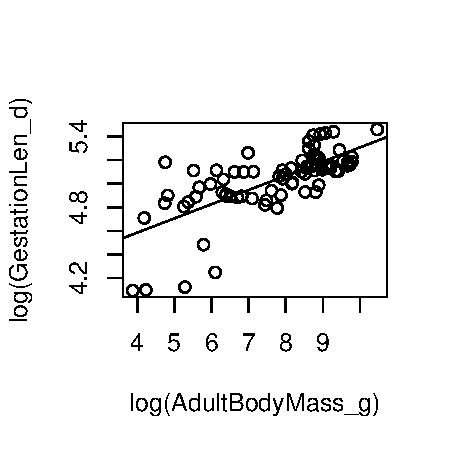
\includegraphics[width = 30cm, height = 10cm, keepaspectratio=true]{OLSplot.pdf}
\caption{Plot of OLS regression model}
\label{figure}
\end{figure}
 
We can look at the phylogenetic pseudoreplication problem on the graph by looking at just one family.

\begin{snugshade}
\begin{Highlighting}[]
\KeywordTok{points}\NormalTok{(}\KeywordTok{log}\NormalTok{(GestationLen_d[Family ==}\StringTok{ "Cercopithecidae"}\NormalTok{]) ~}
      \StringTok{ }\KeywordTok{log}\NormalTok{(AdultBodyMass_g[Family ==}\StringTok{ } \StringTok{"Cercopithecidae"}\NormalTok{]), }
       \DataTypeTok{data =} \NormalTok{primatedata, }\DataTypeTok{col =} \StringTok{"blue"}\NormalTok{, }\DataTypeTok{pch =} \DecValTok{16}\NormalTok{)}
\end{Highlighting}
\end{snugshade}

\subsection{Phylogenetic generalised least squares models (PGLS)}
Phylogenetic generalized least squares (PGLS) models offer some important advantages over independent contrasts. The model of trait evolution can be more flexible i.e., it can depart from a strict Brownian motion process ($\lambda$ or K = 1). Different scaling parameters ($\lambda$, $\kappa$, and $\delta$) can be incorporated in the analysis, which can significantly improve the fit of the data to the model and thus also improve the estimation of the trait correlation. Another advantage of PGLS is that the intercept of the regression is not forced to be zero.

To perform PGLS models in R \texttt{caper} requires you to first combine the phylogeny and data into one object:

\begin{snugshade}
\begin{Highlighting}[]
\NormalTok{primate <-}\StringTok{ }\KeywordTok{comparative.data}\NormalTok{(}\DataTypeTok{phy =} \NormalTok{primatetree, }\DataTypeTok{data =} \NormalTok{primatedata, }
                            \DataTypeTok{names.col =} \NormalTok{Binomial, }\DataTypeTok{vcv =} \OtherTok{TRUE}\NormalTok{, }
                            \DataTypeTok{na.omit =} \OtherTok{FALSE}\NormalTok{, }\DataTypeTok{warn.dropped =} \OtherTok{TRUE}\NormalTok{)}
\end{Highlighting}
\end{snugshade}

\texttt{vcv = TRUE} stores a variance covariance matrix of your tree. You will need this for the \texttt{pgls} function. \texttt{na.omit = FALSE} stops the function from removing species without data for certain variables. \texttt{warn.dropped = TRUE} will tell you if any species are not in the tree and the data and are therefore dropped from the comparative data object. Note that here we will be dropping the 149 species from the tree that we don't have any data for, but we won't drop any species from the data. You can view the dropped species using:

\begin{snugshade}
\begin{Highlighting}[]
\NormalTok{primate\$dropped\$tips}
\NormalTok{primate$dropped$unmatched.rows}
\end{Highlighting}
\end{snugshade}

\begin{framed}
Always make sure you check the list of dropped species is what you expected, it often reveals typos in your species names, or mismatches in taxonomies used etc.
\end{framed}

The function for PGLS analyses in \texttt{caper} is \texttt{pgls}. To fit a model which uses the maximum likelihood estimate of $\lambda$ we use the following code:

\begin{snugshade}
\begin{Highlighting}[]
\NormalTok{model.pgls <-}\StringTok{ }\KeywordTok{pgls}\NormalTok{(}\KeywordTok{log}\NormalTok{(GestationLen_d) ~}\StringTok{ }\KeywordTok{log}\NormalTok{(AdultBodyMass_g), }
                   \DataTypeTok{data =} \NormalTok{primate, }\DataTypeTok{lambda =} \StringTok{"ML"}\NormalTok{)}
\KeywordTok{summary}\NormalTok{(model.pgls)}
\end{Highlighting}
\end{snugshade}

\newpage
The output should look like this:

\begin{verbatim}
## 
## Call:
## pgls(formula = log(GestationLen_d) ~ log(AdultBodyMass_g), 
##      data = primate, lambda = "ML")
## 
## Residuals:
##      Min       1Q   Median       3Q      Max 
## -0.09890 -0.01166  0.00308  0.01776  0.07513 
## 
## Branch length transformations:
## 
## kappa  [Fix]  : 1.000
## lambda [ ML]  : 0.892
##    lower bound : 0.000, p = 1.1e-14
##    upper bound : 1.000, p = 0.00046
##    95.0% CI   : (0.753, 0.967)
## delta  [Fix]  : 1.000
## 
## Coefficients:
##                      Estimate Std. Error t value Pr(>|t|)    
## (Intercept)            4.2902     0.1604   26.75  < 2e-16 ***
## log(AdultBodyMass_g)   0.1049     0.0196    5.34  9.5e-07 ***
## ---
## Signif. codes:  0 '***' 0.001 '**' 0.01 '*' 0.05 '.' 0.1 ' ' 1
## 
## Residual standard error: 0.0261 on 75 degrees of freedom
## Multiple R-squared: 0.276,   Adjusted R-squared: 0.266 
## F-statistic: 28.5 on 1 and 75 DF,  p-value: 9.48e-07
\end{verbatim}

As well as the standard regression outputs, the output includes the estimated ML value of lambda (0.892) and p values from likelihood ratio tests showing whether the ML lambda is significantly different from 0 or 1. Kappa and delta are also tree transformations which can improve the fit of the data to the tree. It is also possible to use \texttt{pgls} to optimise kappa or delta (using delta = "ML" or kappa = "ML" instead of lambda = "ML" in the code above). We will not cover this today but please ask if you want to know more. Note that optimising more than one of these parameters at the same time is not advisable because it would be impossible to interpret the results!

\newpage
We can also plot the results as follows:

\begin{snugshade}
\begin{Highlighting}[]
\KeywordTok{plot}\NormalTok{(}\KeywordTok{log}\NormalTok{(GestationLen_d) ~}\StringTok{ }\KeywordTok{log}\NormalTok{(AdultBodyMass_g), }\DataTypeTok{data =} \NormalTok{primate\$data)}
\KeywordTok{abline}\NormalTok{(model.pgls)}
\end{Highlighting}
\end{snugshade}

\begin{figure}[H]
\centering
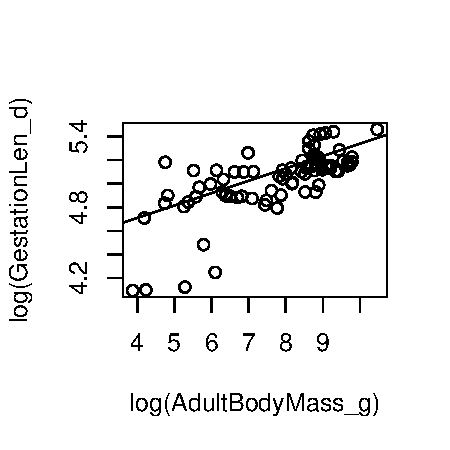
\includegraphics[width = 12cm, height = 12cm, keepaspectratio=true]{PGLSplot.pdf}
\caption{Plot of PGLS regression model}
\label{figure}
\end{figure}

\begin{framed}
Sometimes you will find that \texttt{pgls} will not work and you get an \texttt{optim error}. This is much more common when using a Mac. To fix it all you need to do is change the bounds (upper and lower values) on the parameter being optimised, in this case lambda. Just change the lower bound of lambda to something a little bigger than 1e-6 until it works. For example:

\begin{snugshade}
\begin{Highlighting}[]
\NormalTok{model.pgls2 <-}\StringTok{ }\KeywordTok{pgls}\NormalTok{(}\KeywordTok{log}\NormalTok{(GestationLen_d) ~}\StringTok{ }\KeywordTok{log}\NormalTok{(AdultBodyMass_g), }
                    \DataTypeTok{data =} \NormalTok{primate, }\DataTypeTok{lambda =} \StringTok{"ML"}\NormalTok{, }
                    \DataTypeTok{bounds =} \KeywordTok{list}\NormalTok{(}\DataTypeTok{lambda =} \KeywordTok{c}\NormalTok{(}\FloatTok{1e-05}\NormalTok{, }\DecValTok{1}\NormalTok{)))}
\end{Highlighting}
\end{snugshade}
\end{framed}

\subsection{Likelihood profiles for $\lambda$ in PGLS models}

You can look at the likelihood profiles for branch length transformations in PGLS models using \texttt{pgls.profile}:

\begin{snugshade}
\begin{Highlighting}[]
\NormalTok{lambda.profile <-}\StringTok{ }\KeywordTok{pgls.profile}\NormalTok{(model.pgls, }\StringTok{"lambda"}\NormalTok{)}
\KeywordTok{plot}\NormalTok{(lambda.profile)}
\end{Highlighting}
\end{snugshade}

\begin{figure}[H]
\centering
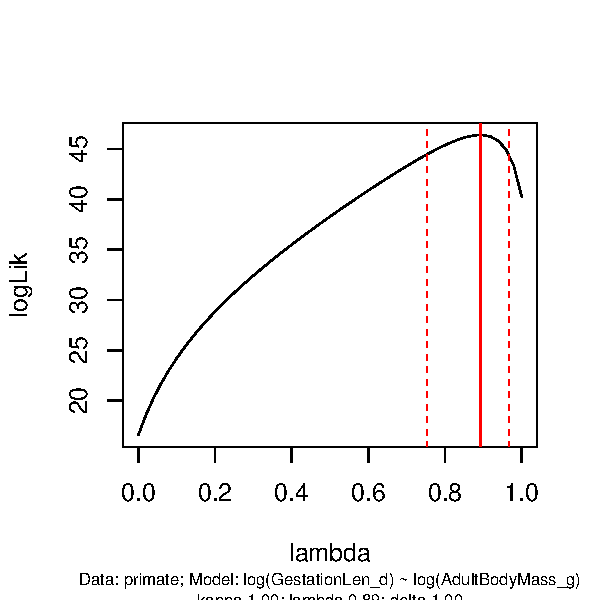
\includegraphics[width = 30cm, height = 10cm, keepaspectratio=true]{lambdaplot.pdf}
\caption{$\lambda$ profile for PGLS model}
\label{figure}
\end{figure}

This graph shows the likelihood profile of $\lambda$ in our model. Ideally you want a line with an obvious peak/optimum like this, rather than a flat line which would suggest $\lambda$ could be anything. You can see that the optimum (the peak of the curve) is at 0.892 as estimated in our PGLS model. The dotted red lines are the 95\% confidence intervals on $\lambda$ for our model. \texttt{pgls.confint} prints out these numbers in \texttt{\$ci.val}

\begin{snugshade}
\begin{Highlighting}[]
\KeywordTok{pgls.confint}\NormalTok{(model.pgls, }\StringTok{"lambda"}\NormalTok{)}\NormalTok{\$ci.val}
\end{Highlighting}
\end{snugshade}

\begin{verbatim}
## [1] 0.7534 0.9665
\end{verbatim}

\begin{framed}
\textbf{Big problems with small datasets}\\

You will often find strange $\lambda$ profiles when you don't have a lot of species in your data, because $\lambda$ (and Blomberg's K - see below) has no power to detect phylogenetic signal for less than 20-30 data points (see Freckleton \textit{et al}. 2002 Am Nat). This means that using PGLS on small datasets is tricky - you almost always get ML $\lambda$ of zero but the $\lambda$ profile will show a pretty flat likelihood surface. Unfortunately people often forget to look at the $\lambda$ profile so erroneously conclude that there is no phylogenetic autocorrelation in their data.

Generally I'd say don't use small datasets, however, this seems unavoidable in many areas of anthropology. Therefore my advice is to (only in this situation!) ignore one of Freckleton's deadly sins (2009, JEB) and report the results from an OLS model (equivalent of PGLS with lambda = 0) and also report the results from a PGLS model with lambda set to 1 (equivalent to independent contrasts). This problem comes up every year at AnthroTree and consensus among the PCM community (well Rob Freckleton, Charlie Nunn and others!) is that this is best solution at present, if collecting more data is really not an option!

To set $\lambda$ to 1 you just replace "ML" with 1:

\begin{snugshade}
\begin{Highlighting}[]
\NormalTok{model.pgls <-}\StringTok{ }\KeywordTok{pgls}\NormalTok{(}\KeywordTok{log}\NormalTok{(GestationLen_d) ~}\StringTok{ }\KeywordTok{log}\NormalTok{(AdultBodyMass_g), }
                   \DataTypeTok{data =} \NormalTok{primate, }\DataTypeTok{lambda =} \StringTok{1}\NormalTok{)}
\end{Highlighting}
\end{snugshade}
\end{framed}

\subsection{Model diagnostics for PGLS models}

You should always check model diagnostic plots whenever you fit a model in R to check that your data meet the assumptions of the model. The method for this in PGLS is the same for OLS, independent contrasts and PGLS models (though the graphs are slightly different). To get model diagnostic plots for PGLS:

\begin{snugshade}
\begin{Highlighting}[]
\KeywordTok{par}\NormalTok{(}\DataTypeTok{mfrow =} \KeywordTok{c}\NormalTok{(}\DecValTok{2}\NormalTok{, }\DecValTok{2}\NormalTok{))}
\KeywordTok{plot}\NormalTok{(model.pgls)}
\end{Highlighting}
\end{snugshade}

\begin{figure}[H]
\centering
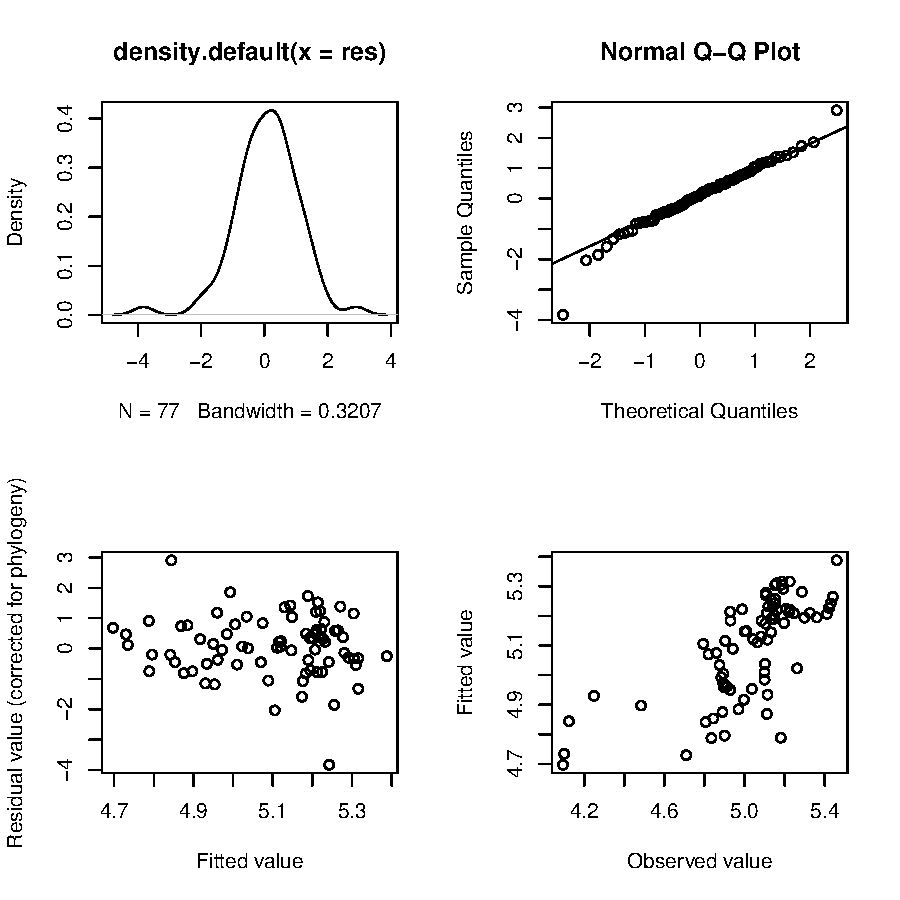
\includegraphics[width = 40cm, height = 12cm, keepaspectratio=true]{Diagnosticplot.pdf}
\caption{Model diagnostic plots for PGLS model}
\label{figure}
\end{figure}

Without going into the statistical details, what you are looking for in these plots is:
\begin{enumerate}
\item No studentized model residuals > $\pm$ 3. 
Any species with such large residuals should be removed as these outliers may overly influence the results of the regression (see Jones and Purvis 1997). Often these are the result of measurement error associated with species pairs joined by very short branches. You should generally report results with and without outliers unless the results remain qualitatively the same.
\item The points of the Q-Q plot should approximately form a straight line (rather than a banana shape).
\item Plots 3 and 4 should show a fairly random scattering of points. You want to avoid any clear patterns.
\end{enumerate}

It takes practice to know what is ``good'', ``bad'' and ``acceptable'' with these plots. I would say the plots above are fine, but there appear to be a couple of outliers that should be removed, or at least checked for errors. 

\subsection{Estimating phylogenetic signal for one variable: $\lambda$}
Phylogenetic signal is merely the pattern where close relatives have more similar trait values than more distant relatives. Often people will mention that they corrected for phylogeny because of the phylogenetic signal in their variables. However, we \texttt{do not} correct for phylogeny because our variables show phylogenetic signal. We correct for phylogeny because the \texttt{residuals} from our models show phylogenetic signal – see Revell 2010 Methods in Ecology and Evolution. $\lambda$ shown in PGLS models below is the $\lambda$ for the model residuals \textbf{not} the individual variables. Also see Kamilar and Cooper 2013 Phil Trans B.

Sometimes however, you might be interested in the phylogenetic signal of just one trait. $\lambda$ is really easy to estimate using \texttt{caper}. To do this for log GestationLen\_d:

\begin{snugshade}
\begin{Highlighting}[]
\NormalTok{est.lambda <-}\StringTok{ }\KeywordTok{pgls}\NormalTok{(}\KeywordTok{log}\NormalTok{(GestationLen_d) ~}\StringTok{ }\DecValTok{1}\NormalTok{, }\DataTypeTok{data =} \NormalTok{primate, }\DataTypeTok{lambda =} \StringTok{"ML"}\NormalTok{)}
\KeywordTok{summary}\NormalTok{(est.lambda)}
\end{Highlighting}
\end{snugshade}

\begin{verbatim}
## 
## Call:
## pgls(formula = log(GestationLen_d) ~ 1, data = primate, lambda = "ML")
## 
## Residuals:
##      Min       1Q   Median       3Q      Max 
## -0.12835 -0.01446  0.00139  0.01757  0.07433 
## 
## Branch length transformations:
## 
## kappa  [Fix]  : 1.000
## lambda [ ML]  : 0.948
##    lower bound : 0.000, p = <2e-16
##    upper bound : 1.000, p = 0.03 
##    95.0% CI   : (0.859, 0.996)
## delta  [Fix]  : 1.000
## 
## Coefficients:
##             Estimate Std. Error t value Pr(>|t|)    
## (Intercept)    5.005      0.117    42.7   <2e-16 ***
## ---
## Signif. codes:  0 '***' 0.001 '**' 0.01 '*' 0.05 '.' 0.1 ' ' 1
## 
## Residual standard error: 0.0334 on 76 degrees of freedom
## Multiple R-squared:    0,    Adjusted R-squared:    0 
## F-statistic:  NaN on 0 and 76 DF,  p-value: NA
\end{verbatim}

Note that by replacing the explanatory variables with 1 you are just investigating the relationship between log gestation length and the phylogeny. Thus the $\lambda$ value is the $\lambda$ estimate for log GestationLen\_d and the p values are from likelihood ratio tests showing whether the ML $\lambda$ is significantly different from 0 (no phylogenetic signal) or 1 (the expectation under Brownian motion).

\subsection{Estimating phylogenetic signal for one variable: Blomberg's K}

To estimate Blomberg’s K we use the \texttt{Kcalc} function in \texttt{picante}. First you need to set up a new vector with the values for the variable you are interested in, here the log of gestation length, and with a names attribute with the names of your species. Here I'll call this vector \texttt{lngest}.

\begin{snugshade}
\begin{Highlighting}[]
\NormalTok{lngest <-}\StringTok{ }\KeywordTok{log}\NormalTok{(primatedata\$GestationLen_d)}
\KeywordTok{names}\NormalTok{(lngest) <-}\StringTok{ }\NormalTok{primatedata\$Binomial}
\end{Highlighting}
\end{snugshade}

We can then calculate K for log gestation length:

\begin{snugshade}
\begin{Highlighting}[]
\KeywordTok{Kcalc}\NormalTok{(lngest[primatetree\$tip.label], primatetree)}
\end{Highlighting}
\end{snugshade}

\begin{verbatim}
## [1] "Dropping taxa from the data because they are not present in the phylogeny:"
## [1] NA
## [1] "Dropping tips from the tree because they are not present in the data:"
##   [1] "Allenopithecus_nigroviridis"                  
##   [2] "Cercopithecus_cephus_cephus"                  
##   [3] "Cercopithecus_cephus_ngottoensis"             
##   [4] "Cercopithecus_diana"
\end{verbatim}

etc.

Note that we are using the original data and tree here, not the pruned down versions, so lots of tips are being dropped.

\begin{verbatim}
##        [,1]
## [1,] 0.7758
\end{verbatim}

Note that \texttt{Kcalc} (and \texttt{phylosignal}) require the trait data to be in the same order as the tree tip labels. \texttt{lngest[primatetree\$tip.label]} selects gestation lengths from the species in the same order as they are in the tree (square brackets \texttt{[ ]} are used in R to subset data).

K for log gestation length is 0.7758. As with $\lambda$ above, we’re interested in whether the value of K is significantly different from what we’d expect by chance. We can do this using the function \texttt{phylosignal}.This function randomly assigns the trait values to the species and then calculates K. This is repeated 1000 times (if \texttt{reps = 1000}) and the observed value of K is then compared to the randomized values to determine its significance.

\begin{snugshade}
\begin{Highlighting}[]
\KeywordTok{phylosignal}\NormalTok{(lngest[primatetree\$tip.label], primatetree, }\DataTypeTok{reps =} \DecValTok{1000}\NormalTok{)}
\end{Highlighting}
\end{snugshade}

After the warnings about which tips have been dropped, the output looks like this:

\begin{verbatim}
##        K PIC.variance.obs PIC.variance.rnd.mean PIC.variance.P
## 1 0.7758         0.001661               0.01212       0.000999
##   PIC.variance.Z
## 1         -2.281
\end{verbatim}

In this case the observed K is significantly higher than the random values of K (Z = -2.281, p < 0.001, mean of the random values = 0.012). 

\textbf{Note this is a randomization test so your answer will not be identical to mine.}

%\newpage
\section{Practice exercises}
The code above only runs these analyses on a few variables. If you have time, try and run some analyses on the other variables. Here are some example questions to get you started (or you can head straight to testing it on your own data!).

\begin{enumerate}
\item What is $\lambda$ for primate social group size?
\item Make a plot of social group size against home range size. Color the Cebidae in green. 
\item Perform a PGLS of two variables of your choice.
\item Does home range size differ significantly among the different primate genera?
\item What is Blomberg’s K for adult body mass?
\item Plot the primate tree and zoom in on the \textit{Saimiri} genus.
\item Run a PGLS analysis to determine the relationship between social group size and gestation length. How does this differ from the result obtained with an OLS regression? Plot the result.
\end{enumerate}

\end{document}